\documentclass[aps,floatfix,11pt,twocolumn]{revtex4-1}
\usepackage{bm}%bold math
\usepackage{graphicx}
\usepackage{amsmath}
\usepackage{amssymb}
\usepackage{setspace}
\usepackage{epstopdf}
\usepackage{scalerel}
\epstopdfsetup{update} % only regenerate pdf files when eps file is newer
\linespread{1}
\usepackage[export]{adjustbox}

%\newcommand*\bplqt{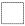
\includegraphics[height=1.6ex] {Symbols/blank_plqt}}
%\newcommand*\bhrzmv{\includegraphics[height=1.6ex]{Symbols/blank_hrzmv}}
%\newcommand*\bdiag{\includegraphics[height=1.6ex] {Symbols/blank_diag}}
%\newcommand*\bstr{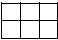
\includegraphics[height=1.6ex] {Symbols/blank_str}}

\newcommand*{\hprs}{%
  \text{% change size in subscripts or superscripts
    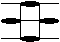
\includegraphics[
      height=1.2ex,% adjust to suit
      valign=M,% center vertically
      raise=\fontdimen22\textfont2,% but raise it to the formula axis
    ]{Symbols/hrzprestar} }
}
\newcommand*{\hspr}{%
  \text{% change size in subscripts or superscripts
    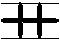
\includegraphics[
      height=1.2ex,% adjust to suit
      valign=M,% center vertically
      raise=\fontdimen22\textfont2,% but raise it to the formula axis
    ]{Symbols/hrzstarpair} }
}

\newcommand*{\bplqt}{%
  \text{% change size in subscripts or superscripts
    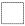
\includegraphics[
      height=1.2ex,% adjust to suit
      valign=M,% center vertically
      raise=\fontdimen22\textfont2,% but raise it to the formula axis
    ]{Symbols/blank_plqt} }
}
\newcommand*{\bhrzmv}{%
  \text{% change size in subscripts or superscripts
    \includegraphics[
      height=1.2ex,% adjust to suit
      valign=M,% center vertically
      raise=\fontdimen22\textfont2,% but raise it to the formula axis
    ]{Symbols/blank_hrzmv} }
}
\newcommand*{\bdiag}{%
  \text{% change size in subscripts or superscripts
    \includegraphics[
      height=1.2ex,% adjust to suit
      valign=M,% center vertically
      raise=\fontdimen22\textfont2,% but raise it to the formula axis
    ]{Symbols/blank_diag} }
}
\newcommand*{\bstr}{%
  \text{% change size in subscripts or superscripts
    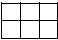
\includegraphics[
      height=1.2ex,% adjust to suit
      valign=M,% center vertically
      raise=\fontdimen22\textfont2,% but raise it to the formula axis
    ]{Symbols/blank_str} }
}
\newcommand*{\vvemptylink}{%
  \text{% change size in subscripts or superscripts
    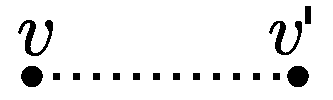
\includegraphics[
      height=1.8ex,% adjust to suit
      valign=M,% center vertically
      raise=\fontdimen22\textfont2,% but raise it to the formula axis
    ]{Symbols/string_net_link_sym0} }
}
\newcommand*{\emptylink}{%
  \text{% change size in subscripts or superscripts
    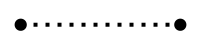
\includegraphics[
      height=1.5ex,% adjust to suit
      valign=M,% center vertically
      raise=\fontdimen22\textfont2,% but raise it to the formula axis
    ]{Symbols/string_net_link_sym1} }
}
\newcommand*{\rightarrowlink}{%
  \text{% change size in subscripts or superscripts
    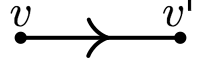
\includegraphics[
      height=1.5ex,% adjust to suit
      valign=M,% center vertically
      raise=\fontdimen22\textfont2,% but raise it to the formula axis
    ]{Symbols/string_net_link_sym2} }
}
\newcommand*{\leftarrowlink}{%
  \text{% change size in subscripts or superscripts
    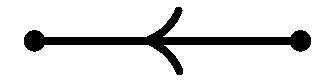
\includegraphics[
      height=1.5ex,% adjust to suit
      valign=M,% center vertically
      raise=\fontdimen22\textfont2,% but raise it to the formula axis
    ]{Symbols/string_net_link_sym3} }
}
\newcommand*{\twointwoout}{%
  \text{% change size in subscripts or superscripts
    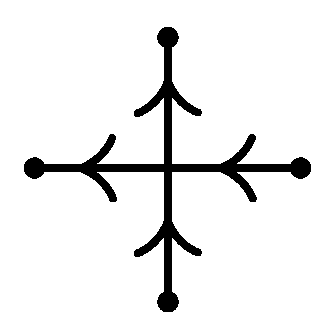
\includegraphics[
      height=1.5ex,% adjust to suit
      valign=M,% center vertically
      raise=\fontdimen22\textfont2,% but raise it to the formula axis
    ]{Symbols/two_in_two_out} }
}
\newcommand*{\oneinoneout}{%
  \text{% change size in subscripts or superscripts
    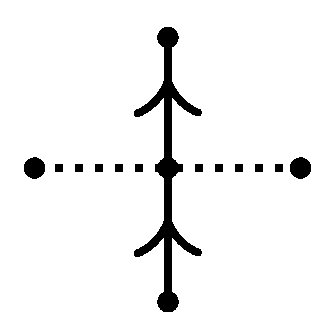
\includegraphics[
      height=1.5ex,% adjust to suit
      valign=M,% center vertically
      raise=\fontdimen22\textfont2,% but raise it to the formula axis
    ]{Symbols/one_in_one_out} }
}
\newcommand*{\threeinzeroout}{%
  \text{% change size in subscripts or superscripts
    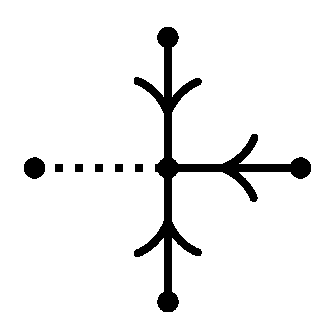
\includegraphics[
      height=1.5ex,% adjust to suit
      valign=M,% center vertically
      raise=\fontdimen22\textfont2,% but raise it to the formula axis
    ]{Symbols/three_in_zero_out} }
}
\newcommand*{\threeoutzeroin}{%
  \text{% change size in subscripts or superscripts
    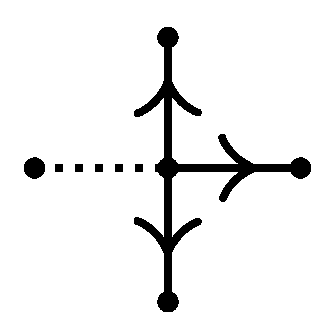
\includegraphics[
      height=1.5ex,% adjust to suit
      valign=M,% center vertically
      raise=\fontdimen22\textfont2,% but raise it to the formula axis
    ]{Symbols/three_out_zero_in} }
}
\newcommand*{\zerooutzeroin}{%
  \text{% change size in subscripts or superscripts
    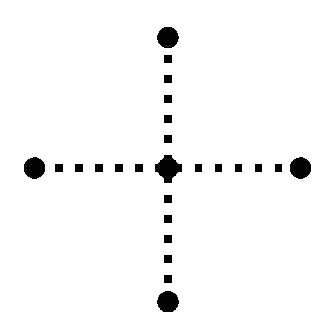
\includegraphics[
      height=1.5ex,% adjust to suit
      valign=M,% center vertically
      raise=\fontdimen22\textfont2,% but raise it to the formula axis
    ]{Symbols/zero_out_zero_in} }
}
\newcommand*{\hrzplqt}{%
  \text{% change size in subscripts or superscripts
    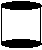
\includegraphics[
      height=1.5ex,% adjust to suit
      valign=M,% center vertically
      raise=\fontdimen22\textfont2,% but raise it to the formula axis
    ]{Symbols/hrzplqt.pdf} }
}
\newcommand*{\vrtplqt}{%
  \text{% change size in subscripts or superscripts
    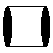
\includegraphics[
      height=1.5ex,% adjust to suit
      valign=M,% center vertically
      raise=\fontdimen22\textfont2,% but raise it to the formula axis
    ]{Symbols/vrtplqt.pdf} }
}

\begin{document}
%%%%%%%%%%%%%%%%%%%%%%%%%%%%%%%%%%%%%%%%%%%%%%%%%%%%%%%%%%%%%%%%%%%%%%%%%%%%%%%%%%%%%%%%%%%%%%%
%%%%%%%%%%%%%%%%%%%%%%%%%%%%%%%%%%%%%%%%%%%%%%%%%%%%%%%%%%%%%%%%%%%%%%%%%%%%%%%%%%%%%%%%%%%%%%%
\section{Introduction}

    It became apparent in the 80's and early 90's that the Landau theory of symmetry breaking did not
    encompass all possible types of order that can be found in the groundstate of a condensed matter system. 
    In fact it was found that the symmetry of a system
    could increase as a system was cooled past a critical tempature and a phase transition occured
    that did not fit into Landau's theory. In these cases the odering 
    that could not be described with an order
    parameters \cite{wen_1990} was a topological order. Though the discovery of topological order was originally thought
    to help understand superconductivity in the context of chiral spin systems \cite{HERE} it was
    not able to do so. However, due to the robust ground state degeneracy of systems exhibiting
    topological order they have become candidates for methods of storing and manipulating
    quantum information.  Also important to the field of quantum information, but interesting in
    its own right, is that topologically ordered systems exhibit fractal excitations. 

    One of the simplest and most well studied models that exhibits topological order is the
    toric code, an exactly solvable model. Unfortunately it is
    a difficult model to physically realize. Another class of models that are well studied are
    the quantum dimer models (QDM).  These models can exhibit topological order and are also
    easier to experimentally realize, for example some short range resonating valence bond
    systems can be approximated with a QDM that provides a low energy effective description of
    the frustrated spins. Some correlation functions in QDMs are solvable using Pfaffian models
    but in general they must be studied numerically. 

    In this paper we numerically study the quantum dimer pentamer model (QDPM) on the square
    lattice at the RK point.  The QDPM contains an exact $Z_3$ local gauge symmetry due to the
    introduction of pentamer objects and we believe it exhibits $Z_3$ topological order.
    Pentamers are objects consisting of four dimers touching a vertex.  The Hilbert space
    comprises all fully packed dimer and pentamer coverings. The presence or absence of a dimer
    may be defined in terms of Ising degrees of freedom that live on the links of the square
    lattice and this distinguishes it from the $Z_3$ toric code with three degrees of freedom on
    the links. We show numerically that a liquid dimer pentamer phase exists at the RK point
    with exponentially decaying dimer correlations. We also estimate the dimer and vison gaps
    showing that the $Z_3$ visons are the lowest lying and most fundamental excitations.

\section{Background}

    Now we will introduce the toric code on the square lattice in some detail to sever as a point of reference and
    comparison for the following discussion of the $Z_3$ case. The toric code Hamiltonian is given by
    %
    \begin{equation}
        H_t = -J_e\sum_v A_v - J_m\sum_p B_p
        \label{eqn:toric_code_ham}
    \end{equation}
    %
    where the operator $A_v$ acts on the vertex $v$ and the sum over $v$ is the sum over all vertices. 
    The operator $B_p$ acts on a plaquette $p$ and the sum over $p$ is the sum over all
    plaquettes. In the $Z_2$ toric code, Ising degrees of freedom live on the links of the
    lattice. Explicitly the operators $A_v$ and $B_p$ can be expressed as
    %
    \begin{equation}
        A_v = \prod_{i\in v} \sigma^x_i
        ,
    \end{equation}
    %
    and
    \begin{equation}
        B_p = \prod_{i\in p} \sigma^z_i
        .
    \end{equation}
    %
    The products are over the links adjacent to vertex $v$ and on the edges of plaquette $p$ for
    $A_v$ and $B_p$ respectively. Since all $A_v$ operators commute with each other, all
    $B_p$ operators commute with each other and $A_v$ commutes with $B_p$ even if they share
    links (commute because they
    can only share an even number of links) then the Hamiltonian can be solved term by term.

    Without a rigorous solution it is possible to guess at the form of the Toric code
    ground state wave function. The first term in \ref{eqn:toric_code_ham} is maximized ($H_t$
    minimized) when an even number of links touching a vertex are spin up or down in the
    $\sigma^z$ basis. By coloring the links of all down spins the groundstate will
    contain closed loops. The second term in \ref{eqn:toric_code_ham} is maximized for a
    superposition of loops since $B_p$ flips the spins around a plaquette $p$. The ground state
    wave function is then a superposition of all possible closed loop configurations. 
    %Since $B_p$ is a local operator
    %though the alowed loop configurations are determined by how the sytem in initilized.
    
    NEED HERE Some stuff about plaquette flux ?? -> $B_p | \Psi \rangle = | \Psi \rangle$ -> only true if
    grnd state as no vortices

    NEED HERE String operators. The electric and magnetic string operators are respectively
    \begin{equation}
        S^e_{\Gamma} = \prod_{i\in\Gamma_e} \sigma^x_i
        ,
    \end{equation}
    \begin{equation}
        S^m_{\Gamma} = \prod_{i\in\Gamma_m} \sigma^z_i
        ,
    \end{equation}
    where the path is denoted by $\Gamma$. The path of the electric string operator is along the
    links of the lattice and if this path is not closed then the operator
    creates a pair of excitations. These excitations are defects in the system 
    that can be thought of as electric charges that live at the
    end of the unclosed string. Each of these electric defects has an energy costs of $2J_e$. 
    The path of the magnetic string operator runs perpendicular to the links
    and starts and ends on the dual lattice. An unclosed magnetic path results in two magnetic
    excitations on the at the ends of the magnetic string each costing $2J_m$ each. 

    Using a nontrivial path (genus of system $>0$) one can move between topological sectors using $S_e$ and determine
    the topological sector the system is in using $S_m$. On a torus, acting with $S_e$ along a
    path that encloses either the major or minor axis of the torus changes the topological sector.
    In general there are $4^g$ topological sectors where $g$ is the
    genus of the system. For a torus then there are four topological sectors. If These can be
    measuerd using the $S_m$ operator on a ...




    \subsection{$Z_3$ Toric Code}
        We can represent the $Z_3$ algebra through the following expressions
        %
        %Z_N
        %\begin{equation}
        %    E |n\rangle = n |n\rangle, ~ n=0,1,2,...,N-1
        %    \\
        %    e^{iA} |n\rangle = |n+1 \rangle, ~ n=0,1,2,...,N-2
        %    \\
        %    e^{iA} |N-1\rangle = |0\rangle
        %    %\label{eqn:}
        %\end{equation}
        %Z_3
        %
        \begin{equation}
            \begin{split}
            & E_l |n_l\rangle = n_l |n_l\rangle, ~ n_l=0,1,2
            \\
            & e^{iA_l} |n_l \rangle = |n_l+1 \rangle, ~ n_l =0,1
            \\ 
            & e^{iA_l} |2 \rangle = |0\rangle
            \end{split}
            ,
            %\label{eqn:}
        \end{equation}
        %
        where the operators $E_l$ and $A_l$ act on a given link $l$ and are analogous to the electric field and vector potential
        respectively. 
        By assigning orientations to the links between two vertices we can define 3 unique
        link ``values'' pictorially. 
        %
        \begin{itemize}
            \item $\vvemptylink$ 
            \item $\rightarrowlink$ 
            \item $\leftarrowlink$ 
        \end{itemize}
        % 
        In this way we can define $e^{iA_l}$ as the operator $Q$ which acts on the links in the
        following way
        \begin{equation}
            \begin{split}
                & Q^\dagger_{vv'}  | \vvemptylink \rangle = | \rightarrowlink \rangle
                ,
                \\
                & Q^\dagger_{vv'}  | \rightarrowlink \rangle = | \leftarrowlink \rangle
                ,
                \\
                & Q^\dagger_{vv'}  | \leftarrowlink \rangle = | \emptylink \rangle
                ,
            \end{split}
            %\label{eqn:}
        \end{equation}
        where the link is specified by the two vertices it connects and the operator
        $Q^\dagger_{vv'}$ acts in a direction from vertex $v$ to vertex $v'$. By changing the
        direction in which $Q$ operates we can express it in terms of its hermitian conjugate. 
        %
        \begin{equation}
            (Q^\dagger_{vv'})^\dagger = Q_{vv'}^\dagger
            .
            %\label{eqn:}
        \end{equation}

        The operator $E$ The operator $E_{vv'}$ can be defined in a similar way as
        %
        \begin{equation}
            \begin{split}
                & E^\dagger_{vv'}  | \vvemptylink \rangle = 0
                ,
                \\
                & E^\dagger_{vv'}  | \rightarrowlink \rangle = | \rightarrowlink \rangle
                ,
                \\
                & E^\dagger_{vv'}  | \leftarrowlink \rangle = 2| \leftarrowlink \rangle
                ,
            \end{split}
            %\label{eqn:}
        \end{equation}
        and with it we can define.
        %
        \begin{equation}
            P_{vv'}^\dagger \equiv e^{i2\pi E_{vv'}/3}
            .
            %\label{eqn:}
        \end{equation}
        %
        Now how $P_{vv'}^\dagger$ acts on the links: 
        %
        \begin{equation}
            \begin{split}
                & P^\dagger_{vv'}  | \vvemptylink \rangle = | \vvemptylink \rangle
                ,
                \\
                & P^\dagger_{vv'}  | \rightarrowlink \rangle = e^{i2\pi/3} | \rightarrowlink \rangle
                ,
                \\
                & P^\dagger_{vv'}  | \leftarrowlink \rangle = e^{-i2\pi/3} | \leftarrowlink \rangle
                .
            \end{split}
            %\label{eqn:}
        \end{equation}
        %

        The $Z_3$ toric code Hamiltonian can now be written in terms of the $P$ and $Q$ operators. The
        usual string net Hamiltonian is written as 
        \begin{equation}
            H = - J_e \sum_v A_v - J_m \sum_p B_p
            %\label{eqn:}
        \end{equation}
        where the sum over $v$ and the sum over $p$ are the sums over all vertices and plaquettes on
        the lattice respectively and 
        \begin{equation}
            A_v = \prod_{i\in v} P^\dagger_{vv_i}~,~ B_p \prod_{i\in p} Q^\dagger_{v_iv_{i+1}}
            .
            %\label{eqn:}
        \end{equation}
        The specific vertex and plaquette labeling scheme is shown in Fig.~\ref{fig:vertex_link_labels}.
        %
        \begin{figure}[htpb]
            \centering
            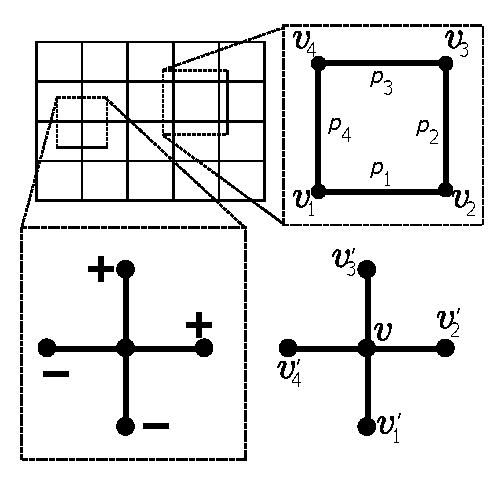
\includegraphics[width=0.8\linewidth]{vertex_link_gauge_def}
            \caption{Notation of vertex and plaquette labels}
            \label{fig:vertex_link_labels}
        \end{figure}
        %
        For the ground state of this Hamiltonian there is a local symmetry corresponding to the
        minimization of the first term. The model has an exactly local gauge symmetry that can be
        expressed as
        \begin{equation}
            G_v | \psi \rangle= | \psi \rangle
            %\label{eqn:}
        \end{equation}
        where $G_v$ = $A_v$.


        \subsubsection{Hamiltonian Gauge symmetry }


        \subsubsection{String operators}
            With the above notation we can write down the string operators. The electric string operator along
            the path $\Gamma_{v_b v_e}$ between the two vertices $v_0$ (beginning) and $v_N$ (end) is written
            %
            \begin{equation}
                S^e_{\Gamma} = \prod_{l=0}^{N-2} Q_{v_lv_{l+1}}^\dagger
                %\label{eqn:}
                ,
            \end{equation}
            %
            where $v_l \in \Gamma$ and $N$ is the number of vertices in $\Gamma$. We show an example of an
            electric string operator operation on an example configuration in Fig.~\ref{fig:example_elec_string}.
            %
            %
            \begin{figure}[htpb]
                \centering
                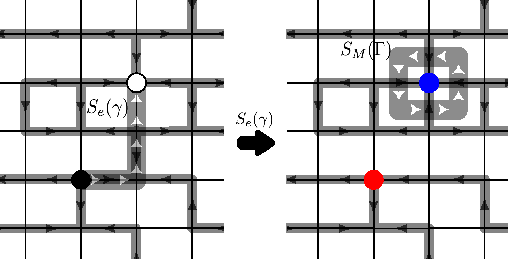
\includegraphics[width=0.8\linewidth]{example_elec_string.pdf}
                \caption{The grey line is the path $\Gamma$ on which the string operator acts. The operator acts
            in the direction from the vertex labeled in red to the one labeled in blue.}
                \label{fig:example_elec_string}
            \end{figure}
            %
            %
            The magnetic string operator can be written as
            \begin{equation}
                S^m_{\Gamma} = \prod_{l=0}^{N-1} Q_{v_{2l}v_{2l+1}}^\dagger
                %\label{eqn:}
            \end{equation}
            %
            where $v_l$ are the vertices adjacent to the links in $\Gamma$ and $N$ is the number of
            vertices
            on the \textit{left} side of the path when looking along the path from red to blue. 
            An example of this operator acting
            on a configuration is shown in Fig.~\ref{fig:example_mag_string} along with the vertex labeling
            scheme.
            %
            %
            \begin{figure}[htpb]
                \centering
                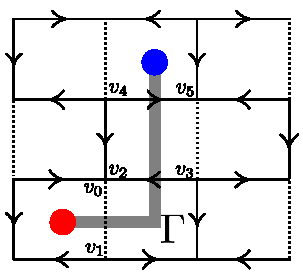
\includegraphics[width=0.8\linewidth]{example_mag_string.pdf}
                \caption{The grey line is the path $\Gamma$ on which the string operator acts. The magnetic
                    string operator acts in the 
                    direction from the plaquette labeled in red to the one labeled in blue.}
                \label{fig:example_mag_string}
            \end{figure}
            %
            The magnetic string operator acting on path $\Gamma$ in Fig.~\ref{fig:example_mag_string} is
            explicitly
            %
            \begin{multline}
                S^m_{\Gamma} (\mathrm{~Fig.~\ref{fig:example_mag_string}~config})
                = P_{v_0v_1}^\dagger P_{v_2v_3}^\dagger P_{v_4v_5}^\dagger
                \\
                = \exp{[0 - \frac{i2\pi}{3} + \frac{i2\pi}{3} ]} 
                = 1 (\mathrm{~Fig.~\ref{fig:example_mag_string}~config})
                .
            \end{multline}
            %

            An interesting property of the electric string string operators in the $Z_3$ toric code is
            that they produce two defects, one having positive charge and the other having negative
            charge. This is most easily see by looking at Fig.~\ref{fig:example_elec_string}. The
            configuration in Fig.~\ref{fig:example_elec_string}(a) obeys the local gauge symmetry and
            when the electric string operator acts on path $\Gamma$ it results in two defects at the
            end points of $\Gamma$. At the first $v_0$ (red) the local constraint is broken and
            $G_{v_0} = e^{i2\pi /3}$ as shown in Fig.~\ref{fig:example_elec_string}(b), whereas
            $G_{v_3} = e^{-i2\pi /3}$ which can be thought of as negative and positive gauge charges
            at $v_0$ and $v_3$ respectively.

            The magnetic excitations, or $Z_3$ visons live at the endpoints of a path created with the magnetic
            string operator. These visons can take three different values which can be changed by
            operating with the electric operator on a path that encircles one endpoint of the
            magnetic string path. 


        \subsubsection{properties of $Z_3$ string operators}

        \subsubsection{Winding Numbers}

            The ground state of the $Z_3$ toric code on the torus is nine-fold degenerate because of
            the nine different topological sectors in this topology. One can move between the
            topological sectors with a nontrivial closed electric string wraps around either
            the major axis or the minor axis of the torus. We will call the electric winding
            operator that acts around the major axis $W^e_y$ and around the minor axis $W^e_x$.
            A given topological sector can be distinguish 
            by acting around the minor and major axes with the magnetic string operator $W^m_y$ and
            $W^m_x$. All of the aforementioned winding operators commute with the Hamiltonian and
            therefore share the same eigenvalues. The operator $W^m_{x}$ ($W^m_{y}$) can 
            have three different values depending on how many electric strings enclose the minor
            (major) axis. Since there are three different
            possible values for each winding number around each axis there are nine distinct
            topological sectors.


    \subsection{QDM on Square lattice}
        Here we will review the relevant
        properties and attributes of the QDM on the square lattice for which the Hamiltonian is.
        \begin{equation}
            \label{}
            H_{\mathrm{QDM}} = -t\sum_{\bplqt} 
                \left(
                    \left|
                        \vrtplqt
                    \right\rangle
                    \left\langle
                        \hrzplqt
                    \right|
                    +
                    \mathrm{h.c.}
                \right)
            - v\sum_{\bplqt}
                \left(
                    \left|
                        \vrtplqt
                    \right\rangle
                    \left\langle
                        \vrtplqt
                    \right|
                    +
                    \left|
                        \hrzplqt{}
                    \right\rangle
                    \left\langle
                        \hrzplqt
                    \right|
                \right)
                .
        \end{equation}
        This model can be defined in terms of a single parameter $t/v$ for which the wave function is
        known exactly at the Rokhsar and Kivelson (RK) point, the point where $t/v =1$. At the RK
        point the wave function is the equal weighted superposition over all dimer configurations.
        HERE



%%%%%%%%%%%%%%%%%%%%%%%%%%%%%%%%%%%%%%%%%%%%%%%%%%%%%%%%%%%%%%%%%%%%%%%%%%%%%%%%%%%%%%%%%%%%%%%
%%%%%%%%%%%%%%%%%%%%%%%%%%%%%%%%%%%%%%%%%%%%%%%%%%%%%%%%%%%%%%%%%%%%%%%%%%%%%%%%%%%%%%%%%%%%%%%
\section{The Quantum Dimer Pentamer Model}

    \subsection{Local $Z_3$ Gauge Symmetry}

        In the QDPM Ising degrees of freedom live on the links of the lattice.
        The operator $\hat{\sigma}^x_l$ acts on these links and has 
        eigenvalues $\sigma_l = \pm 1$, where $\sigma_l$ is the
        Ising variables of the $l^{\mathrm{th}}$ link on the lattice. The number operator for a give link is
        defined as $\hat{n}_l \equiv (1+\hat{\sigma}_x)/2$ and counts the number of dimers on link $l$.
        An exactly local gauge symmetry exists on the lattice due to the constraint that either one or
        four dimers touch any give vertex. In terms of $n_l$ we can define an operator that counts the
        number of dimers touching a given vertex $v$ as $n_v = \sum_{l\in v} n_l$. 
        
        the local gauge transformation $G_v$ acting on a give vertex $v$ for the quantum dimer model
        can be expressed as
        %
        \begin{equation}
            \label{}
            G_v=e^{i \alpha (n_v - n_0)}
        \end{equation}
        %
        where $n_0$ is the constrained number of dimers touching a vertex, $n_0=1$ in the QDM model,
        The operator $G_v$ then acts in such a
        way that only the physical states, states satisfying the local constraint 
        are invariant. For the QDM $G_v =
        e^{i\alpha (0)}$ and therefore $G_v$ leaves a physical state unchanged for any
        $\alpha$ making the local gauge symmetry $U(1)$. The local gauge transformation that leaves
        only configurations containing dimers and pentamers invariant is
        %
        \begin{equation}
            \label{eqn:gauge_trans}
            G_v = e^{i (\hat{n}_v -1) 2\pi/3}    
        \end{equation}
        %
        For the QDPM $\alpha$ is must be $2\pi/3$ due to the relaxed constraint of the QDM
        model that allows for pentamers. Relaxing the constraint of the QDM brings the local gauge
        symmetry from $U(1)$ to $Z(3)$.

    \subsection{QDPM Hamiltonian}

        We work specifically at the RK point at which the ground state wave function
        is an equal weighted superposition of fully packed dimer pentamer configurations
        %
        \begin{equation}
            \label{}
            \left| \Psi \right\rangle = \frac{1}{\sqrt{N}}\sum_{\{C\}} \left| C \right\rangle
            ,
        \end{equation}
        %
        where $\{C\}$ is the set of fully packed configurations. The Hilbert space can be defined
        using the gauge transformation in Eq.~\ref{eqn:gauge_trans} as all $\left| C \right\rangle$
        satisfying $G \left| C \right\rangle = \left| C \right\rangle$.

        The QDPM Hamiltonian
        \begin{equation}
            H_{\mathrm{QDPM}} = H_{\mathrm{QDM}} + \mathrm{pentamer\ terms}
        \end{equation}

        The pentamer terms in the Hamiltonian can be constructed with the dynamics shown in
        Fig.~\ref{fig:pentamer_moves}.  
        \begin{figure}[htpb]
            \centering
            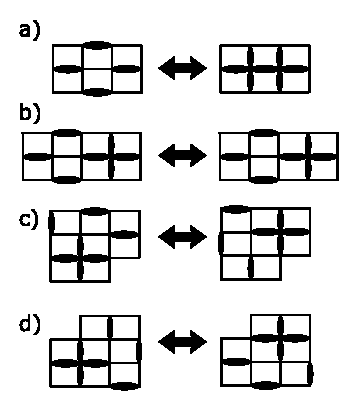
\includegraphics[width=0.8\linewidth]{pentamer_moves.pdf}
            \caption{a) Horizontal creation an annihilation, b) horizontal move, c) and d) are two
            different possible diagonal moves in the same direction.}
            \label{fig:pentamer_moves}
        \end{figure}
        Each of the  moves shown in Fig.~\ref{fig:pentamer_moves} can be
        rotated to produce the symmetry related counterpart (eg. vertical creation and annihilation). 
        As an example the creation and annihilation term in the Hamiltonian is
        \begin{multline}
        H_{\mathrm{pentamer\ creation}} = t_{\mathrm{create}}
            \sum_{\bstr}
            \left(
                \left|
                    \hprs
                \right\rangle
                \left\langle
                    \hspr
                \right|
                +
                \mathrm{h.c.}
            \right)
            \\
            - v_{\mathrm{create}}
            \sum_{\bstr}
                \left(
                    \left|
                        \hprs
                    \right\rangle
                    \left\langle
                        \hprs
                    \right|
                    +
                    \left|
                        \hspr
                    \right\rangle
                    \left\langle
                        \hspr
                    \right|
                \right)
        \end{multline}
        where the factors $t_{\mathrm{create}}$ and $v_{\mathrm{create}}$ are the coefficients of
        the pentamer pair creation and annihilation respectively. At the RK point
        $t/v=1$ for each all the pentamer terms. 
        Writing the kinetic and potential energy terms as done above for all the dynamics shown in
        Fig.~\ref{fig:pentamer_moves} and all of their symmetry related counterparts comprise the
        the pentamer terms of the Hamiltonian. 

    \subsection{Winding operators}

        In the QDPM there is a conserved winding operator in a given topological sector
        \begin{equation}
            W_{x,y} = (N_A - N_B)\mod{3} = n
            .
        \end{equation}
        For $W_y$ ($W_x$), $N_A$ is the number of dimers crossed on a vertical (horizontal) cut and
        $n=0$, $1$, or $2$ depending on the topological sector. The winding operator commutes with
        the Hamiltonian and therefore share the same eigenvalues. Since there are three winding numbers in
        each direction then the ground state is ninefold degenerate.

%%%%%%%%%%%%%%%%%%%%%%%%%%%%%%%%%%%%%%%%%%%%%%%%%%%%%%%%%%%%%%%%%%%%%%%%%%%%%%%%%%%%%%%%%%%%%%%
%%%%%%%%%%%%%%%%%%%%%%%%%%%%%%%%%%%%%%%%%%%%%%%%%%%%%%%%%%%%%%%%%%%%%%%%%%%%%%%%%%%%%%%%%%%%%%%
\section{Dimer Correlation Results}

    \subsection{Liquid}


    \subsection{Correlation functions}

    \begin{equation}
        C_{\mathrm{dimer}} = \langle d_0 d_r \rangle - \langle d_0 \rangle   \langle d_r \rangle   
    \end{equation}

    \begin{figure}[htpb]
        \centering
        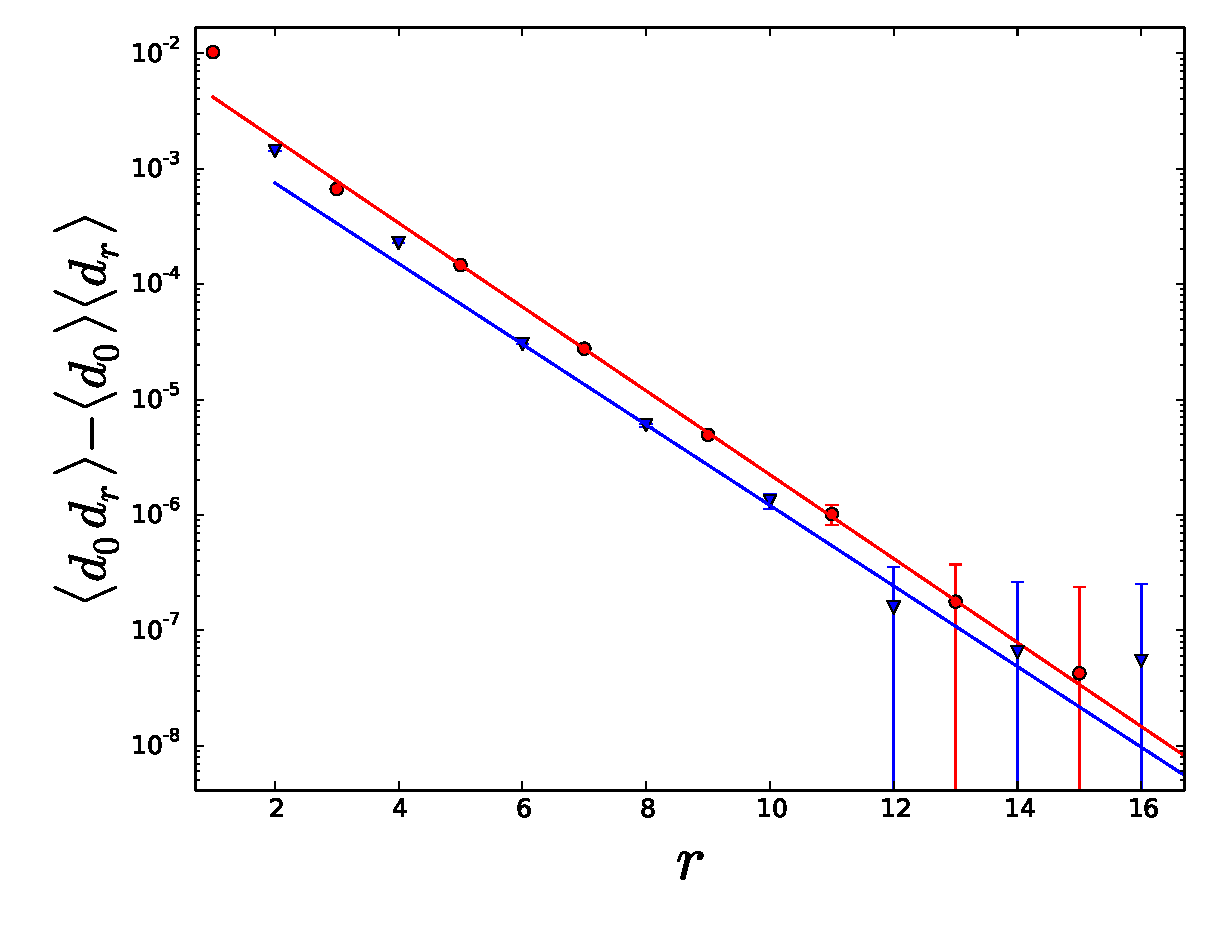
\includegraphics[width=0.8\linewidth]{spacial_dmr_cor.pdf}
        \caption{(Note: This figure was made using equal probabilities of plaquette flips and
        pentamer moves) Spacial correlation function of parallel dimers for the two different
        sublattices distinguished by their color (red, green).}
        \label{fig:spacial_dmr_cor}
    \end{figure}

    \subsection{Comparison to other models}

%%%%%%%%%%%%%%%%%%%%%%%%%%%%%%%%%%%%%%%%%%%%%%%%%%%%%%%%%%%%%%%%%%%%%%%%%%%%%%%%%%%%%%%%%%%%%%%
%%%%%%%%%%%%%%%%%%%%%%%%%%%%%%%%%%%%%%%%%%%%%%%%%%%%%%%%%%%%%%%%%%%%%%%%%%%%%%%%%%%%%%%%%%%%%%%
\section{Estimating the Gap}

    \begin{table}[htpb]
        \centering
        \caption{$\Delta \tau = 150$}
        \label{tab:label}
        \begin{tabular}{c c c}
            \hline\hline
         L            & 8x8 Gap                            & 16x16  \\ 
            \hline
         frac 1.0     &                                    & \\
            \hline
         Dimer &  $ 0.03230 \pm 0.01142$            & $0.00806 \pm 0.00023$ \\
         $Z_2$ origin &  $ 0.00787 \pm 5.3\times 10^{-6} $ & $0.00198 \pm 3.8\times 10^{-6} $   \\
         $Z_3$ origin &  NA                                & NA \\
            \hline
         frac 0.9     &                                    & \\
            \hline
         Dimer origin &  $ 0.00419 \pm 8.1\times 10^{-6} $ & $0.00429 \pm 6.6\times 10^{-6} $ \\
         $Z_2$ origin &  $ 0.00216 \pm 1.5\times 10^{-6} $ & $0.00129 \pm 1.8\times 10^{-6} $  \\
         $Z_3$ origin &  $ 0.00346 \pm 3.8\times 10^{-6} $ & $0.00359 \pm 3.5\times 10^{-6} $ \\
            \hline
         frac 0.5     &                                    & \\
            \hline
         Dimer origin &                                    & $0.02049 \pm 0.00011 $\\
         $Z_2$ origin &                                    & $0.00614 \pm 2.8\times 10^{-6} $ \\
         $Z_3$ origin &                                    & $0.01927 \pm 0.00002 $ 
        \end{tabular}
    \end{table}





    \subsection{Imaginary time vison correlations}
    \begin{figure}[htpb]
        \centering
        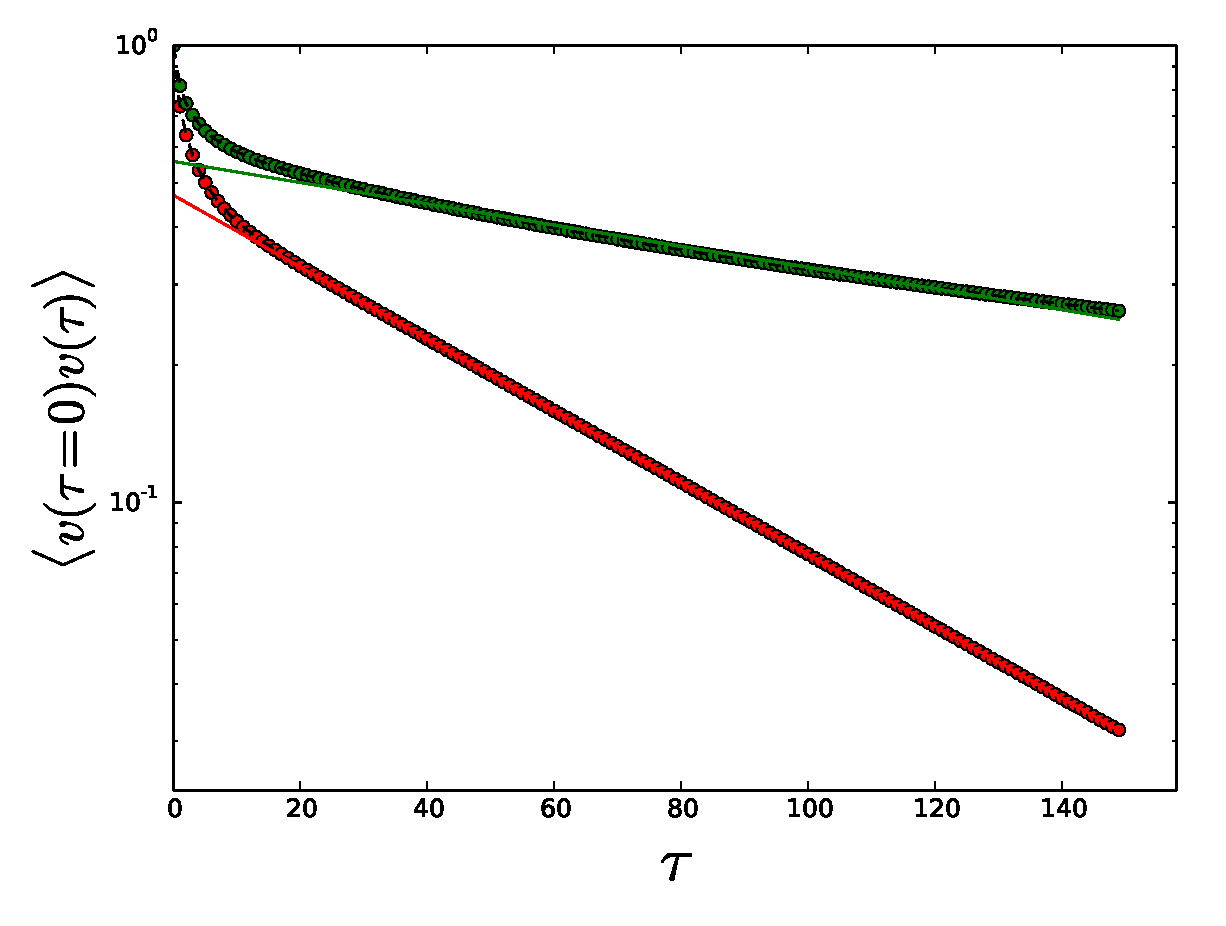
\includegraphics[width=0.8\linewidth]{z2_origin_vison_time_cor.pdf}
        \caption{Imaginary time $z_2$ \textit{single} vison correlations at the origin in the QDM model (red) and QDPM
        model (green) on an $8\times8$ lattice. For the QDPM the dimer/pentamer move fraction is $0.9$.}
        \label{fig:name}
    \end{figure}

    \subsection{Imaginary time dimer correlations}
    \begin{figure}[htpb]
        \centering
        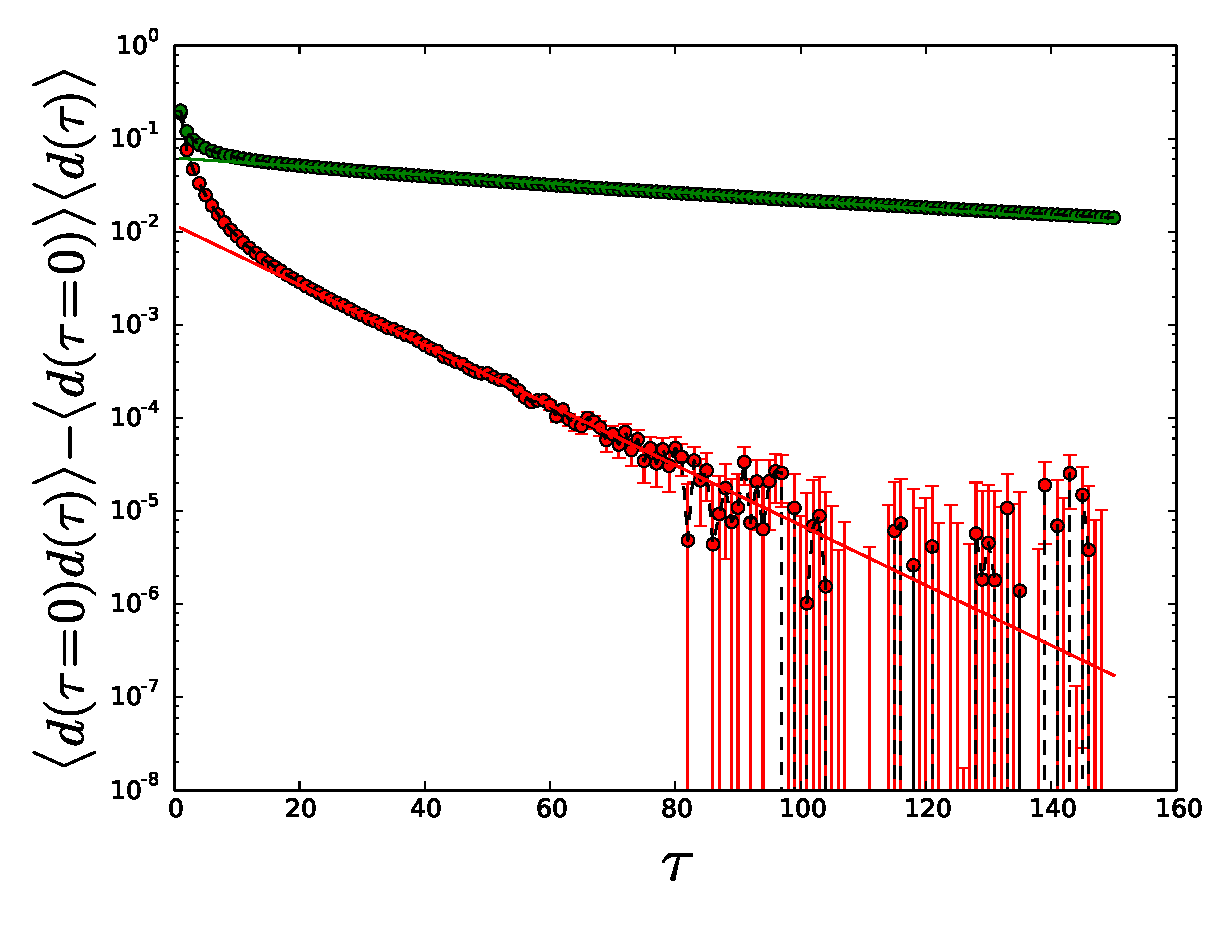
\includegraphics[width=0.8\linewidth]{dimer_origin_time_cor.pdf}
        \caption{Imaginary time dimer correlations of a single dimer in the QDM model (red) and QDPM
        model (green) on an $8\times8$ lattice. For the QDPM the dimer/pentamer move fraction is $0.9$. }
        \label{fig:}

    \end{figure}

%%%%%%%%%%%%%%%%%%%%%%%%%%%%%%%%%%%%%%%%%%%%%%%%%%%%%%%%%%%%%%%%%%%%%%%%%%%%%%%%%%%%%%%%%%%%%%%
%%%%%%%%%%%%%%%%%%%%%%%%%%%%%%%%%%%%%%%%%%%%%%%%%%%%%%%%%%%%%%%%%%%%%%%%%%%%%%%%%%%%%%%%%%%%%%%
\section{Discussion}

\end{document}
